\documentclass[11pt]{article}
\usepackage[margin=1.05in]{geometry}
\usepackage{amsmath,amssymb}
\usepackage{graphicx}
\usepackage{booktabs}
\usepackage{xcolor}
\usepackage[colorlinks=true,linkcolor=blue!55!black,urlcolor=blue!55!black]{hyperref}
\usepackage{microtype}

\title{Study Notes: the Epicycle and the Vortical-Shwave Density\\
\large Derivations behind the Phase-0 PI-question analyses\\
(companion to \texttt{pi\_questions\_analysis.ipynb})}
\author{}
\date{2026-08-19}

\newcommand{\dd}{\mathrm{d}}
\begin{document}
\maketitle

\noindent These notes collect, in print form, the two derivations written into the
PI-questions notebook: (\S\ref{sec:epi}) the epicycle equations of motion and the
reference solution used against the \texttt{epi\_unif}/\allowbreak
\texttt{epi\_ring}/\allowbreak\texttt{epi\_bndry} runs, and (\S\ref{sec:shw}) the envelope physics of the
vortical-shwave density --- why it peaks at the swing and decays afterwards ---
verified parameter-free against a fine-cadence rerun. \S\ref{sec:shw_deriv} adds a
step-by-step derivation of the linearized shearing-wave system itself, including
how the background advection $-q\Omega x\,\partial_y$ becomes the time-dependent
radial wavenumber $k_x(t)$. Conventions follow the code:
$q \equiv -\dd\ln\Omega/\dd\ln R$ ($=3/2$ Keplerian), background azimuthal flow
$v_y = -q\Omega x$.

%=====================================================================
\section{The epicycle: equations of motion and the reference solution}
\label{sec:epi}

\subsection{The shearing-sheet frame and its two forces}
Work in a small Cartesian patch co-rotating with the disk at radius $R_0$ with
angular frequency $\Omega \equiv \Omega(R_0)$: $x = R - R_0$ (radial),
$y = R_0(\phi - \Omega t)$ (azimuthal), $z$ vertical. Two inertial/gravity terms
survive at first order in $x/R_0$.

\paragraph{Tidal term.} The effective potential in the rotating frame is
$\Phi_{\rm eff}(R) = \Phi(R) - \tfrac12\Omega^2R^2$. Circular-orbit balance gives
$\dd\Phi/\dd R = R\,\Omega^2(R)$, and the local power law $\Omega \propto R^{-q}$
gives $\Omega^2(R_0{+}x) \simeq \Omega^2\,(1 - 2q\,x/R_0)$. Expanding to first
order in $x$,
\begin{equation}
\frac{\dd\Phi_{\rm eff}}{\dd R}\bigg|_{R_0+x}
 = (R_0{+}x)\,\Omega^2(R_0{+}x) - \Omega^2(R_0{+}x)\,\big|_{\rm centrifugal}
 = -2q\,\Omega^2 x + O(x^2/R_0),
\end{equation}
i.e.\ a radial force $+2q\Omega^2x\,\hat{\mathbf x}$: tidal stretching, outward
beyond $R_0$ and inward inside. \emph{This expansion is the linearization that
defines the sheet; everything after it is exact within the sheet.}

\paragraph{Coriolis term.} With $\boldsymbol\Omega = \Omega\hat{\mathbf z}$,
$-2\boldsymbol\Omega\times\mathbf v = 2\Omega v_y\,\hat{\mathbf x}
- 2\Omega v_x\,\hat{\mathbf y}$.

\medskip\noindent
The momentum equations of the (unstratified) sheet are therefore
\begin{equation}
\frac{\mathrm{D}v_x}{\mathrm{D}t} = 2\Omega v_y + 2q\Omega^2 x
 - \frac{1}{\rho}\partial_x p,
\qquad
\frac{\mathrm{D}v_y}{\mathrm{D}t} = -2\Omega v_x - \frac{1}{\rho}\partial_y p.
\label{eq:sheet}
\end{equation}

\subsection{Equilibrium}
$v_x = 0$, $v_y = -q\Omega x$ with uniform $\rho, p$ balances exactly:
$2\Omega(-q\Omega x) + 2q\Omega^2x = 0$. This is the background that orbital
advection (FARGO) splits off and advects analytically; the evolved azimuthal
variable is the fluctuation $v_y' \equiv v_y + q\Omega x$.

\subsection{Spatially uniform perturbation: an exact reduction}
Take $v_x = v_x(t)$ and $v_y' = v_y'(t)$ uniform in space (the \texttt{ipert=1}
initial condition: $v_x(0) = A$, $v_y'(0) = 0$), with $\rho$ and $p$ uniform. Then
\begin{itemize}
\item pressure gradients vanish;
\item the fluctuation self-advection $\mathbf v'\!\cdot\!\nabla\mathbf v'$ vanishes
  \emph{identically} --- no linearization in the amplitude $A$ is needed; the only
  surviving advection is $v_x\,\partial_x$ acting on the background $-q\Omega x$;
\item continuity gives $\partial_t\rho = -\nabla\!\cdot(\rho\mathbf v) = 0$: the
  density stays \emph{exactly} $\rho_0$ (the property the Q0.1 interface test
  exploits).
\end{itemize}
Substituting $v_y = -q\Omega x + v_y'$ into Eq.~\eqref{eq:sheet}:
\begin{align}
\dot v_x &= 2\Omega(-q\Omega x + v_y') + 2q\Omega^2 x = 2\Omega\,v_y',
\label{eq:epi_vx}\\
\dot v_y' - q\Omega\,v_x &= -2\Omega\,v_x
\;\;\Longrightarrow\;\;
\dot v_y' = -(2-q)\,\Omega\,v_x ,
\label{eq:epi_vy}
\end{align}
where the $-q\Omega v_x$ on the left is the advection of the background shear.

\subsection{The epicyclic oscillator and the reference solution}
Combining the two equations,
\begin{equation}
\ddot v_x = -\,2(2-q)\,\Omega^2\,v_x \equiv -\kappa^2 v_x,
\qquad
\boxed{\;\kappa^2 = 2(2-q)\,\Omega^2\;}
\end{equation}
the local form of the general epicyclic frequency
$\kappa^2 = R^{-3}\,\dd(R^4\Omega^2)/\dd R = (4-2q)\Omega^2$. For $q = 3/2$:
$\kappa = \Omega$. With the code's initial condition,
\begin{equation}
v_x(t) = A\cos\kappa t,
\qquad
v_y'(t) = \frac{\dot v_x}{2\Omega} = -\frac{A\kappa}{2\Omega}\sin\kappa t .
\end{equation}
The orbit in $(v_x, v_y')$ space is a clockwise ellipse with axis ratio
$\kappa/2\Omega$ ($=1/2$ Keplerian); the displacement
$x(t) = x_0 + (A/\kappa)\sin\kappa t$ is the classical retrograde epicycle.

\subsection{The two diagnostics used against the runs}
\begin{itemize}
\item \textbf{Direct trajectory:} volume-averaged
  $\langle\rho v_x\rangle/\langle\rho\rangle$ vs.\ $A\cos\kappa t$. Envelope
  differences here are dominated by accumulated RK2 \emph{phase} drift.
\item \textbf{Amplitude invariant:} eliminating $t$,
\begin{equation}
\mathcal A(t) \equiv
\sqrt{v_x^2 + \Big(\frac{2\Omega}{\kappa}\Big)^{2} v_y'^{\,2}} = A = \text{const},
\label{eq:invariant}
\end{equation}
conserved by the exact dynamics at \emph{any} amplitude (it is the oscillator
energy in disguise), so its drift isolates numerical damping/growth from phase
error.
\item For short runs the volume-integrated $x$-kinetic energy
  $\int\!\tfrac12\rho v_x^2\,\dd V = \tfrac12\rho_0A^2\cos^2(\kappa t)\,V_{\rm box}$
  is used instead.
\end{itemize}

\subsection{100-orbit results (2026-08-19 reruns)}
\begin{center}\small
\begin{tabular}{@{}lccc@{}}
\toprule
run & $v_x$ range$/A$ & invariant drift & $\max|v_x - A\cos\kappa t|/A$\\
\midrule
uniform $128^2$ & $[-1.00059,\,+1.00045]$ & $+0.321\%$ & $0.124$\\
ring SMR        & $[-1.00001,\,+1.00000]$ & $+0.040\%$ & $0.031$\\
bndry SMR       & $[-1.00001,\,+1.00000]$ & $+0.040\%$ & $0.031$\\
\bottomrule
\end{tabular}
\end{center}
The two SMR runs are bit-identical to each other over all 100 orbits; the
uniformity sweep again gives $\max|\rho-1| = 0.0$ exactly in every float32
snapshot. Both error channels are pure RK2 time integration and scale like it:
the SMR runs integrate the whole domain at half the timestep (global $\Delta t$
set by the fine level), and the measured uniform/SMR ratios are
$0.124/0.031 = 4.0 = (\Delta t_u/\Delta t_s)^2$ for phase error and
$0.321/0.040 = 8.0 = (\Delta t_u/\Delta t_s)^3$ for the invariant drift ---
RK2's per-unit-time phase error is $O(\Delta t^2)$ and its secular amplitude
growth $O(\Delta t^3)$, both derived in \S\ref{sec:rk2} below.

\begin{figure}[htb]
\centering
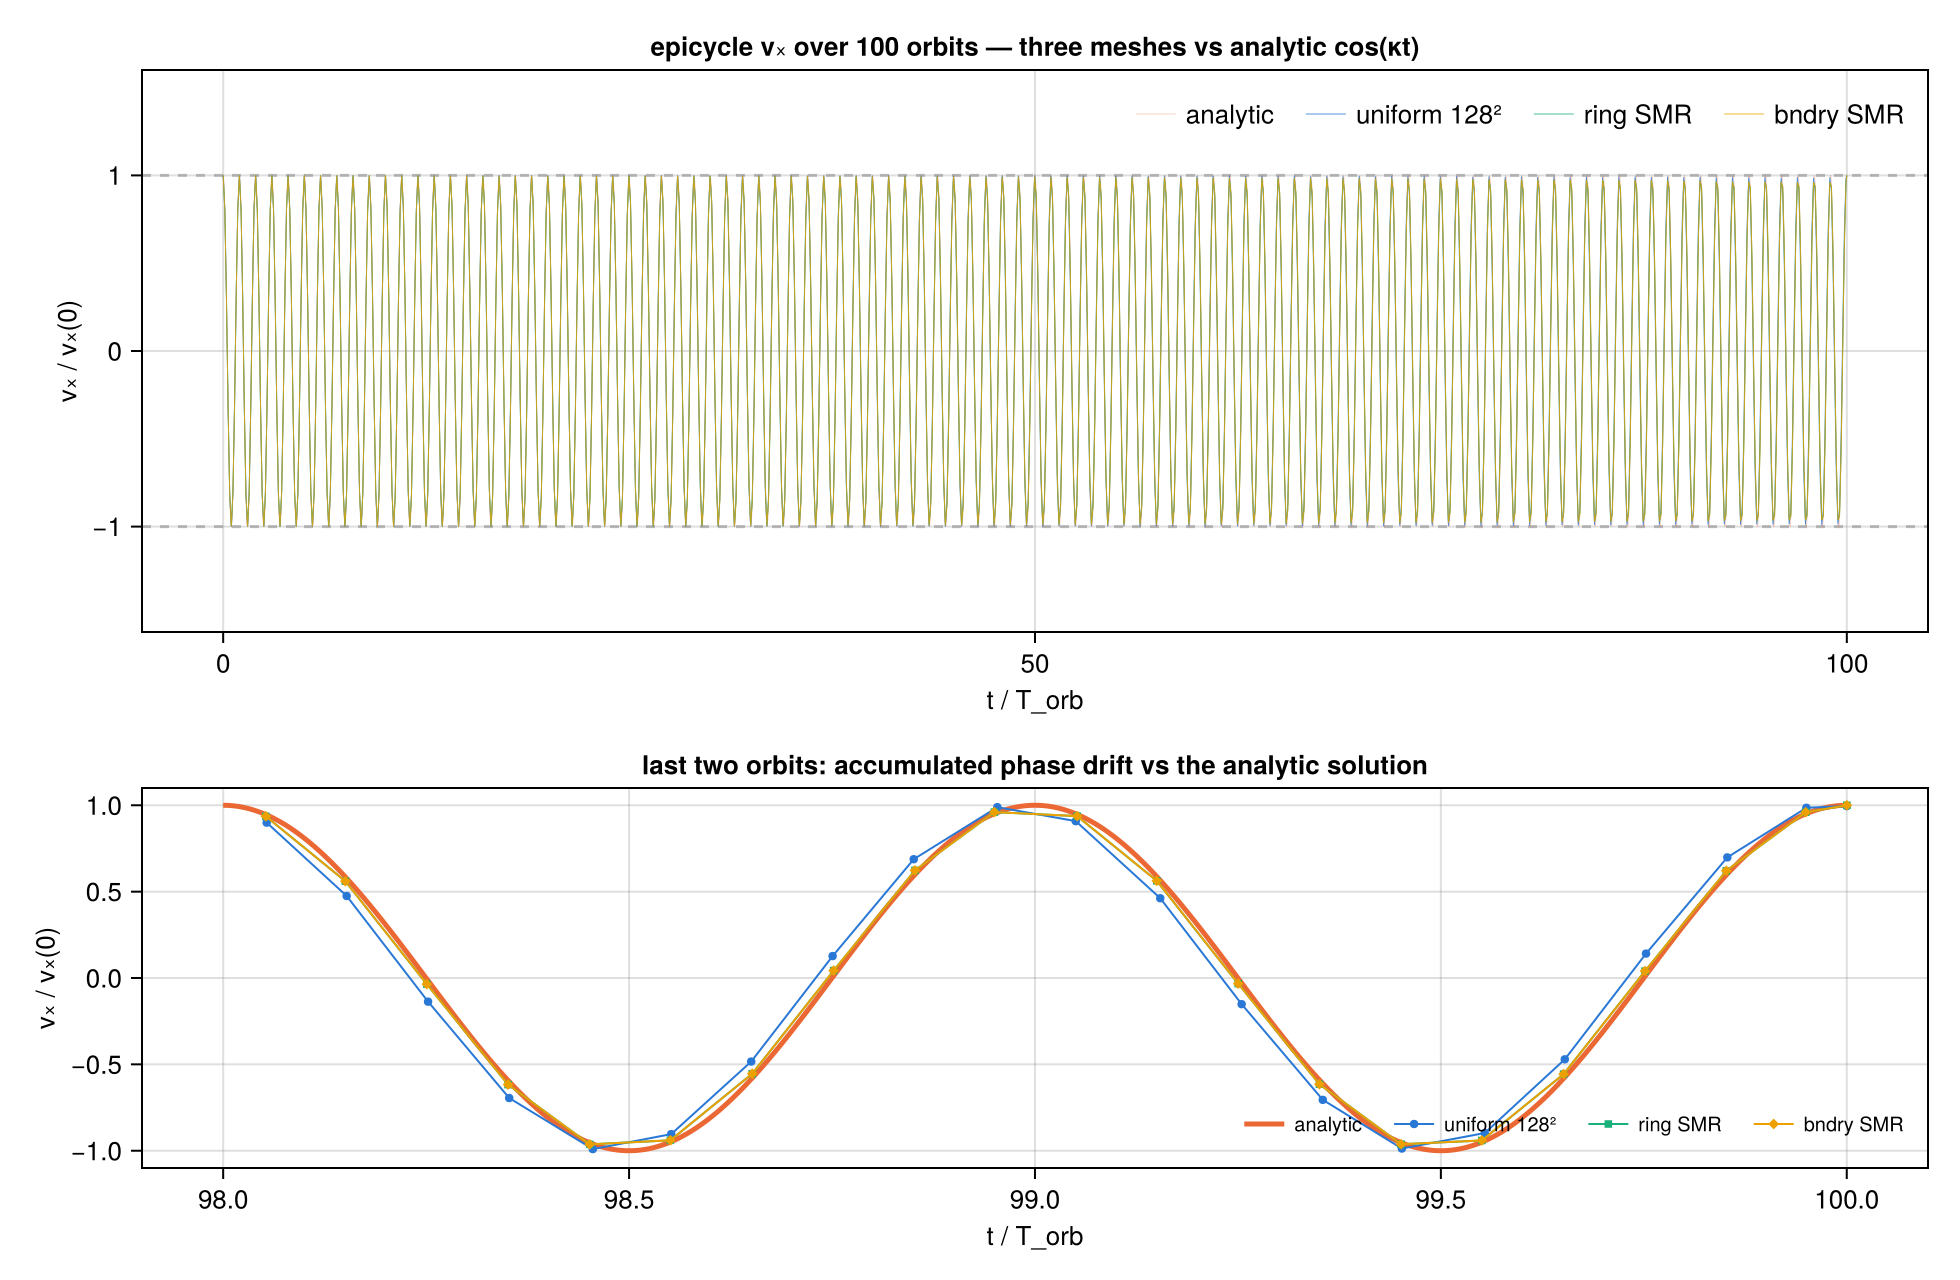
\includegraphics[width=\textwidth]{figures/pi_q01_epi100_vx.png}
\caption{$v_x/v_x(0)$ over 100 orbits for the three meshes vs.\ the analytic
$\cos\kappa t$ (top: full span; bottom: final two orbits). The uniform run leads
in phase by $\sim\!1/8$ period; the two SMR runs overlap (bit-identical) and hug
the analytic curve.}
\label{fig:epi100}
\end{figure}

\subsection{Why the drifts: RK2 on a pure oscillator}
\label{sec:rk2}

\paragraph{Reduction to the model problem.}
Define the complex variable $u = v_x + i\,(2\Omega/\kappa)\,v_y'$. The epicycle
pair (Eqs.~\ref{eq:epi_vx}--\ref{eq:epi_vy}) combines into exactly
\begin{equation}
\dot u = -i\kappa\,u ,
\end{equation}
whose exact solution rotates $u$ on a circle at rate $\kappa$ with $|u|$
constant --- and $|u|$ \emph{is} the amplitude invariant $\mathcal A$ of
Eq.~\eqref{eq:invariant}. ``Invariant drift'' is therefore precisely ``what the
integrator does to $|u|$ per step''. Because the uniform epicycle collapses the
full PDE to this single ODE, the textbook stability analysis below applies to
the simulation \emph{literally}, with no spatial-discretization contamination.

\paragraph{One RK2 step.}
For any linear problem $\dot u = \lambda u$, one step of any two-stage
second-order Runge--Kutta method (Heun, midpoint --- AthenaK's \texttt{rk2}
included) gives exactly
\begin{equation}
u^{n+1} = R(z)\,u^{n}, \qquad R(z) = 1 + z + \tfrac{z^2}{2}, \qquad
z = \lambda\Delta t ,
\end{equation}
the Taylor series of the true propagator $e^{z}$ truncated after the $z^2$
term. The truncation is the whole story.

\paragraph{Amplitude: why growth, and why $(\omega\Delta t)^4/8$.}
Here $z = -i\theta$ with $\theta = \kappa\Delta t$, and the exact propagator
$e^{-i\theta}$ has modulus exactly 1. The truncated polynomial does not:
\begin{equation}
|R|^2 = \Big(1 - \tfrac{\theta^2}{2}\Big)^{2} + \theta^2
      = 1 - \theta^2 + \tfrac{\theta^4}{4} + \theta^2
      = 1 + \tfrac{\theta^4}{4}
\;\;\Longrightarrow\;\;
|R| \simeq 1 + \tfrac{\theta^4}{8} .
\end{equation}
The $\theta^2$ terms cancel exactly (that is what second order buys: forward
Euler has $|R|^2 = 1+\theta^2$), leaving a \emph{positive} remainder: each step
multiplies the amplitude by $1 + (\kappa\Delta t)^4/8 > 1$. Geometrically, the
exact step moves $u$ along the circle; the RK2 step moves it along the parabola
that matches the circle to second order, and a parabola hugging a circle from
outside lands slightly \emph{outside} it --- a tiny energy injection, every
step, always outward. RK2 is weakly \emph{anti-dissipative} on oscillations:
not noise that averages out, but a systematic bias. (RK4's quartic lands
slightly \emph{inside}, $|R_4|^2 = 1 - \theta^6/72 + \ldots$, weak damping;
leapfrog/symplectic schemes land exactly on the circle and err only in phase.)

\paragraph{Accumulation and the $\Delta t^3$ law.}
Per step the relative gain $(\kappa\Delta t)^4/8$ is invisibly small
($1.7\times10^{-7}$ at $\Delta t = 0.0342$), but a run of length $T$ takes
$N = T/\Delta t$ steps and the gains compound with the same sign:
\begin{equation}
\frac{\Delta\mathcal A}{\mathcal A}
= N\,\frac{(\kappa\Delta t)^4}{8}
= \boxed{\;\frac{T\,\kappa^4\,\Delta t^3}{8}\;}
\end{equation}
--- \emph{linear in $T$} (secular; measured: $+0.064\%$ at 20 orbits
$\to$ $+0.321\%$ at 100) and $\propto\Delta t^3$ per unit time (one power of
$\Delta t$ is spent on needing more steps). Halving the step cuts the drift by
$2^3 = 8$: the SMR runs take exactly half the uniform step, and
$0.321/0.040 = 8.0$.

\paragraph{Phase: the same logic, one order earlier.}
The argument of $R$ is also slightly wrong:
$\arg R = -\big(\theta + \theta^3/6 + \ldots\big)$, i.e.\ the numerical
rotation \emph{overshoots} the true angle by $\theta^3/6$ per step --- which is
why the runs \emph{lead} the analytic cosine in Fig.~\ref{fig:epi100}. Accumulated:
$\Delta\varphi = N\,\theta^3/6 = T\kappa^3\Delta t^2/6 \propto \Delta t^2$,
hence the factor $4$ at half the step ($0.124/0.031 = 4.0$).

\paragraph{The formulas predict the absolute numbers.}
With $T = 200\pi$, $\kappa = 1$, and the measured timesteps
($\Delta t = 0.0342$ uniform, $0.0171$ SMR) --- no fitting anywhere:
\begin{center}\small
\begin{tabular}{@{}lcc@{}}
\toprule
quantity & predicted & measured\\
\midrule
uniform invariant drift, $T\kappa^4\Delta t^3/8$ & $+0.315\%$ & $+0.321\%$\\
SMR invariant drift & $+0.039\%$ & $+0.040\%$\\
uniform phase offset, $T\kappa^3\Delta t^2/6$ & $0.123$\,rad & $0.124$\\
SMR phase offset & $0.0307$ & $0.0308$\\
\bottomrule
\end{tabular}
\end{center}
All four agree to $\sim\!2\%$. This is the Q0.1 conclusion from yet another
angle: the entire error budget of these runs is the time integrator behaving
exactly like its textbook analysis --- the mesh, its interfaces, and the shear
machinery contribute nothing measurable.

\clearpage
%=====================================================================
\section{The vortical-shwave density: peaks, nulls, and decay}
\label{sec:shw}

\noindent\emph{Context (Q0.2): the density panels of the shwave comparison movie
flicker frame-to-frame. The flicker is temporal aliasing of the free acoustic
ringing; this section derives the smooth envelope underneath and what sets it.
The derivation is self-contained, but the framework is the ``shwave'' linear
theory of Johnson \& Gammie (2005a), and the test problem is the code-verification
setup of Johnson \& Gammie (2005b, their Fig.~1) --- both in \texttt{docs/}.}

\subsection{Single shearing wave}
Linear isothermal perturbations on the shear, as one shearing wave
$\propto \exp[i(k_x(t)x + k_y y)]$ with
\begin{equation}
k_x(t) = k_{x0} + q\Omega k_y\,t ,
\label{eq:kxt}
\end{equation}
so the shear tilts the wave through the \emph{swing} $k_x = 0$ at
$t_{\rm swing} = -k_{x0}/(q\Omega k_y)$. (Movie configuration:
$64^2$, box $0.5^2$, $c_s = 1$, $(n_{wx}, n_{wy}) = (-8, 2)$, amp $=10^{-4}$,
so $k_{x0} = -32\pi$, $k_y = 8\pi$, $k_x/k_y$ runs $-4 \to 0 \to +3.5$ and
$t_{\rm swing} = 8/3$.) The Fourier amplitudes obey
\begin{equation}
\dot{\hat v}_x = 2\Omega\hat v_y - i k_x c_s^2\hat\delta,\qquad
\dot{\hat v}_y = -(2{-}q)\Omega\hat v_x - i k_y c_s^2\hat\delta,\qquad
\dot{\hat\delta} = -i(k_x\hat v_x + k_y\hat v_y),
\label{eq:shw_odes}
\end{equation}
with $\hat\delta \equiv \widehat{\delta\rho}/\rho_0$ and
$k^2(t) = k_x^2(t) + k_y^2$. The next subsection derives
Eqs.~\eqref{eq:kxt}--\eqref{eq:shw_odes} from the sheet equations; a reader who
takes them as given can skip to \S\ref{sec:pv}.

\subsection{Where the shearing-wave system comes from}
\label{sec:shw_deriv}
\noindent\emph{Derivation of Eqs.~\eqref{eq:kxt}--\eqref{eq:shw_odes} from the
sheet equations.} The only step here that is not routine is how the background
advection
$-q\Omega x\,\partial_y$ --- whose explicit factor of $x$ spoils an ordinary
plane wave --- is absorbed into a \emph{time-dependent} radial wavenumber.

\paragraph{Linearization, term by term.} Add continuity to the sheet momentum
equations~\eqref{eq:sheet} with $p = c_s^2\rho$ (isothermal), and split
$\rho = \rho_0(1+\delta)$, $\mathbf v = \mathbf v^0 + \mathbf v'$ about the
equilibrium $\mathbf v^0 = -q\Omega x\,\hat{\mathbf y}$ of \S1.2, keeping first
order in $(\delta, \mathbf v')$. The advective term contributes three pieces,
\begin{equation}
(\mathbf v\!\cdot\!\nabla)\mathbf v =
\underbrace{(\mathbf v^0\!\cdot\!\nabla)\mathbf v^0}_{=\,0}
+ \underbrace{(\mathbf v^0\!\cdot\!\nabla)\mathbf v'}_{-q\Omega x\,\partial_y\mathbf v'}
+ \underbrace{(\mathbf v'\!\cdot\!\nabla)\mathbf v^0}_{-q\Omega v_x'\,\hat{\mathbf y}}
+ O(v'^2),
\end{equation}
of which the second is advection \emph{of} the perturbation \emph{by} the
background (the term of interest below) and the third is advection of the
background by the perturbation --- it hits only the $y$-equation, because
$\mathbf v^0$ has only a $y$-component, and it is the same term that turned
$-2\Omega$ into $-(2{-}q)\Omega$ in Eq.~\eqref{eq:epi_vy}. In the $x$-equation
the Coriolis and
tidal backgrounds cancel, $2\Omega(-q\Omega x + v_y') + 2q\Omega^2x = 2\Omega
v_y'$ --- that cancellation \emph{is} the equilibrium condition --- and the
pressure gradient linearizes to $-c_s^2\nabla\delta$ (uniform background
pressure, so $1/\rho$ may be evaluated at $\rho_0$). With
$\nabla\!\cdot\!\mathbf v^0 = 0$, continuity gives
$\partial_t\delta - q\Omega x\,\partial_y\delta = -\nabla\!\cdot\!\mathbf v'$.
All three equations therefore carry the \emph{same} linearized advective
operator $\mathrm{D}_t \equiv \partial_t - q\Omega x\,\partial_y$:
\begin{equation}
\mathrm{D}_t v_x' = 2\Omega v_y' - c_s^2\partial_x\delta,
\qquad
\mathrm{D}_t v_y' = -(2{-}q)\Omega v_x' - c_s^2\partial_y\delta,
\qquad
\mathrm{D}_t \delta = -(\partial_x v_x' + \partial_y v_y').
\label{eq:shw_lin}
\end{equation}

\paragraph{Why a fixed-$k$ Fourier mode fails.} For
$f \propto e^{i(k_xx + k_yy)}$ with constant $k_x$, the offending term is
$-q\Omega x\,\partial_y f = -i\,q\Omega k_y\,x\,f$: the explicit $x$ maps the
mode onto $x\times(\text{mode})$, a \emph{different} function, so plane waves are
not eigenfunctions of $\mathrm{D}_t$. Since $x \leftrightarrow i\,\partial/\partial k_x$
under Fourier transform, this term is an advection in $k$-space,
$\partial_t\hat f + q\Omega k_y\,\partial\hat f/\partial k_x = (\text{local
terms})$, whose characteristics are $\dd k_x/\dd t = q\Omega k_y$. Modes drift
along the $k_x$ axis at a fixed rate; the shearing-wave ansatz simply rides that
characteristic.

\paragraph{The shearing-wave ansatz (the load-bearing step).} Put the time
dependence in the wavenumber itself,
$f(x,y,t) = \hat f(t)\,e^{i\varphi}$ with $\varphi = k_x(t)x + k_yy$. Then
$\partial_t$ \emph{at fixed position} picks up two pieces --- the changing
amplitude and the rotating phase --- and
\begin{equation}
\mathrm{D}_t f
= \Big[\dot{\hat f} + i\,\dot k_x x\,\hat f\Big]e^{i\varphi}
  - i\,q\Omega k_y x\,\hat f\,e^{i\varphi}
= \Big[\dot{\hat f} + i\,x\big(\dot k_x - q\Omega k_y\big)\hat f\Big]e^{i\varphi}.
\end{equation}
The $x$-dependent piece --- exactly what broke the fixed-$k$ mode --- vanishes
for \emph{all} $x$ if and only if $\dot k_x = q\Omega k_y$, i.e.\
Eq.~\eqref{eq:kxt}, and then $\mathrm{D}_t f = \dot{\hat f}\,e^{i\varphi}$: the
entire background advection has been absorbed into the drifting wavenumber. The
geometric content is that surfaces of constant phase are \emph{material} surfaces
of the background flow --- along a background trajectory ($x$ fixed,
$y(t) = y_0 - q\Omega x t$),
\begin{equation}
\varphi(t) = (k_{x0} + q\Omega k_yt)\,x + k_y(y_0 - q\Omega x t)
 = k_{x0}x + k_yy_0 = \text{const},
\end{equation}
so ``$\dd/\dd t$ at fixed phase'' is the shear tilting the crests, and tilting
crests \emph{is} winding up $k_x$. Equivalently, in shearing coordinates
$y' = y + q\Omega t\,x$ this is an ordinary Fourier mode
$e^{i(k_{x0}x' + k_yy')}$, and expanding the exponent returns
$k_x(t)x + k_yy$ --- the same relation the FFT solver applies to the transform of
the rolled (sheared-coordinate) density, $k_x^{\rm phys} = k_x' + q\Omega
t\,(L_x/L_y)k_y$, where $k_x', k_y$ are integer mode indices and the $L_x/L_y$ is
the conversion between them.

\paragraph{Collapse to Eq.~\eqref{eq:shw_odes}.} With the ansatz in force,
$\mathrm{D}_t \to \dd/\dd t$, $\partial_x \to ik_x(t)$, $\partial_y \to ik_y$,
and the common factor $e^{i\varphi}$ divides out of
Eq.~\eqref{eq:shw_lin} --- leaving precisely Eq.~\eqref{eq:shw_odes}, with
$\hat v_x, \hat v_y$ the amplitudes of the fluctuations $v_x', v_y'$. These ODEs
are exact within linear theory: no WKB or slowly-varying assumption has been made
(that enters only at Eq.~\eqref{eq:slaved}), and the sole approximation remains
the dropping of $O(v'^2)$.

\paragraph{Two checks.} (i) \emph{Uniform limit}: at $k_{x0} = k_y = 0$ the
pressure and compression terms vanish and Eq.~\eqref{eq:shw_odes} reduces to the
epicycle pair of Eqs.~\eqref{eq:epi_vx}--\eqref{eq:epi_vy} --- \S\ref{sec:epi} is
the $k \to 0$ member of this
family. (ii) \emph{Potential vorticity}: differentiating $\xi$ of
Eq.~\eqref{eq:pv} below and substituting Eq.~\eqref{eq:shw_odes}, the $c_s^2$
terms cancel pairwise and the rotational terms collect to
$ik_y\hat v_y\,[\,q - 2 + (2{-}q)\,]\Omega = 0$ --- but only because
$\dot k_x = q\Omega k_y$, so PV conservation is itself a consistency check on the
ansatz.

\subsection{The carrier: conserved potential vorticity}
\label{sec:pv}
The perturbation potential vorticity
\begin{equation}
\xi \;=\; i\big(k_x\hat v_y - k_y\hat v_x\big) \;-\; (2-q)\,\Omega\,\hat\delta
\label{eq:pv}
\end{equation}
is \emph{exactly} conserved by Eqs.~\eqref{eq:shw_odes} (direct differentiation,
using $\dot k_x = q\Omega k_y$). In the nearly incompressible regime the vortical
wave is $\hat v_x = i k_y\hat\psi$, $\hat v_y = -i k_x\hat\psi$ with
$\xi \simeq k^2\hat\psi$, hence
\begin{equation}
|\mathbf v| = \frac{\xi}{k(t)} :
\end{equation}
the velocity amplitude peaks where $k(t)$ is smallest --- the swing --- and decays
as $1/k \propto 1/t$ afterwards as the shear rewinds the wave to ever finer radial
scale. \textbf{Transient amplification, no instability}: the PV budget is fixed
and merely gets spread over growing $k$. In component form,
$\hat v_x = ik_y\hat\psi = ik_y\,\xi/k^2 \propto (1+\tau^2)^{-1}$ with
$\tau = k_x/k_y$ --- exactly eq.~(9) of Johnson \& Gammie (2005b), the amplitude
law the validation document verifies to $<0.5\%$ of peak on all three meshes.

\subsection{The density: a driven acoustic oscillator}
Differentiating the continuity relation in Eq.~\eqref{eq:shw_odes} once and
substituting the momentum equations,
\begin{equation}
\ddot{\hat\delta} + c_s^2 k^2(t)\,\hat\delta \;=\; S(t),
\qquad
S = -2i\Omega\big[(q{-}1)k_y\hat v_x + k_x\hat v_y\big]
  \;=\; \frac{2\Omega\,\xi\,\big[(q{-}1)k_y^2 - k_x^2(t)\big]}{k^2(t)} ,
\label{eq:oscillator}
\end{equation}
an acoustic oscillator at the instantaneous (WKB) frequency $c_sk(t)$, driven by
the Coriolis/shear forces acting on the vortical flow. Its solution is a
\textbf{slaved response plus free ringing}:
\begin{itemize}
\item \emph{Slaved} (adiabatic; valid since $c_sk \gg \Omega$ throughout):
\begin{equation}
\boxed{\;
\hat\delta_{\rm slv}(t) = \frac{S}{c_s^2k^2}
= \frac{2\Omega\,\xi\,\big[(q{-}1)k_y^2 - k_x^2(t)\big]}{c_s^2\,k^4(t)}\;},
\qquad
\xi = \mathrm{amp}\cdot\frac{k_0^2}{k_y},
\label{eq:slaved}
\end{equation}
with $k_0 = k(0)$ (the pgen's amp is the $v_x$ amplitude).
\item \emph{Free ringing} at $\omega = c_sk(t)$, launched at $t=0$ because the
pgen initializes $\delta\rho = 0$ rather than $\hat\delta_{\rm slv}(0)$ (and
re-pumped near the swing, where the drive varies fastest); WKB amplitude
$\propto k^{-1/2}$. This is what the movie's 0.1-cadence frames undersample
(2.4--2.9 beats of $|\hat\delta|$ per frame at $t \approx 5$), producing the
stroboscopic flicker.
\end{itemize}

\subsection{Envelope anatomy --- all parameter-free}
Writing $u = k_x^2/k_y^2$, Eq.~\eqref{eq:slaved} $\propto |u - (q{-}1)|/(u+1)^2$:
\begin{itemize}
\item a \textbf{local maximum at $k_x = -\sqrt2\,k_y$} ($u = 2$; here $t = 1.72$);
\item \textbf{nulls at $k_x^2 = (q{-}1)k_y^2$} (here $t = 2.20$ and $3.14$): the
tilt angles at which the two Coriolis/shear force projections in $S$ cancel;
\item the \textbf{absolute peak at the swing} ($k_x=0$, $t = 8/3$), where $1/k^4$
is maximal:
$\hat\delta_{\rm peak} = 2\Omega\xi(q{-}1)/(c_s^2k_y^2) = 0.68\times10^{-4}$
for the movie configuration (measured: $0.76\times10^{-4}$, the excess being
ringing on top). The density peaks at the swing for the same reason the velocity
does --- minimum $k$ --- but more sharply ($k^{-4}$ vs.\ $k^{-1}$): pressure
resists compression least when the wave is least wound;
\item \textbf{decay as $t\to\infty$}: the slaved part falls as
$2\Omega\xi/(c_sk_x)^2 \propto t^{-2}$ (stiffening pressure vs.\ weakening
vortical drive), the ringing as $k^{-1/2} \propto t^{-1/2}$, so the late band is
ringing-dominated. On longer horizons the winding drives the radial wavelength to
the grid scale and numerical diffusion ($\propto k^2$) extinguishes everything
super-exponentially. Nothing can grow: without self-gravity there is no feedback
channel (contrast the \texttt{swing\_selfgrav} runs at $4\pi G > 2$, where the
crest grows instead of bouncing).
\end{itemize}

\begin{figure}[htb]
\centering
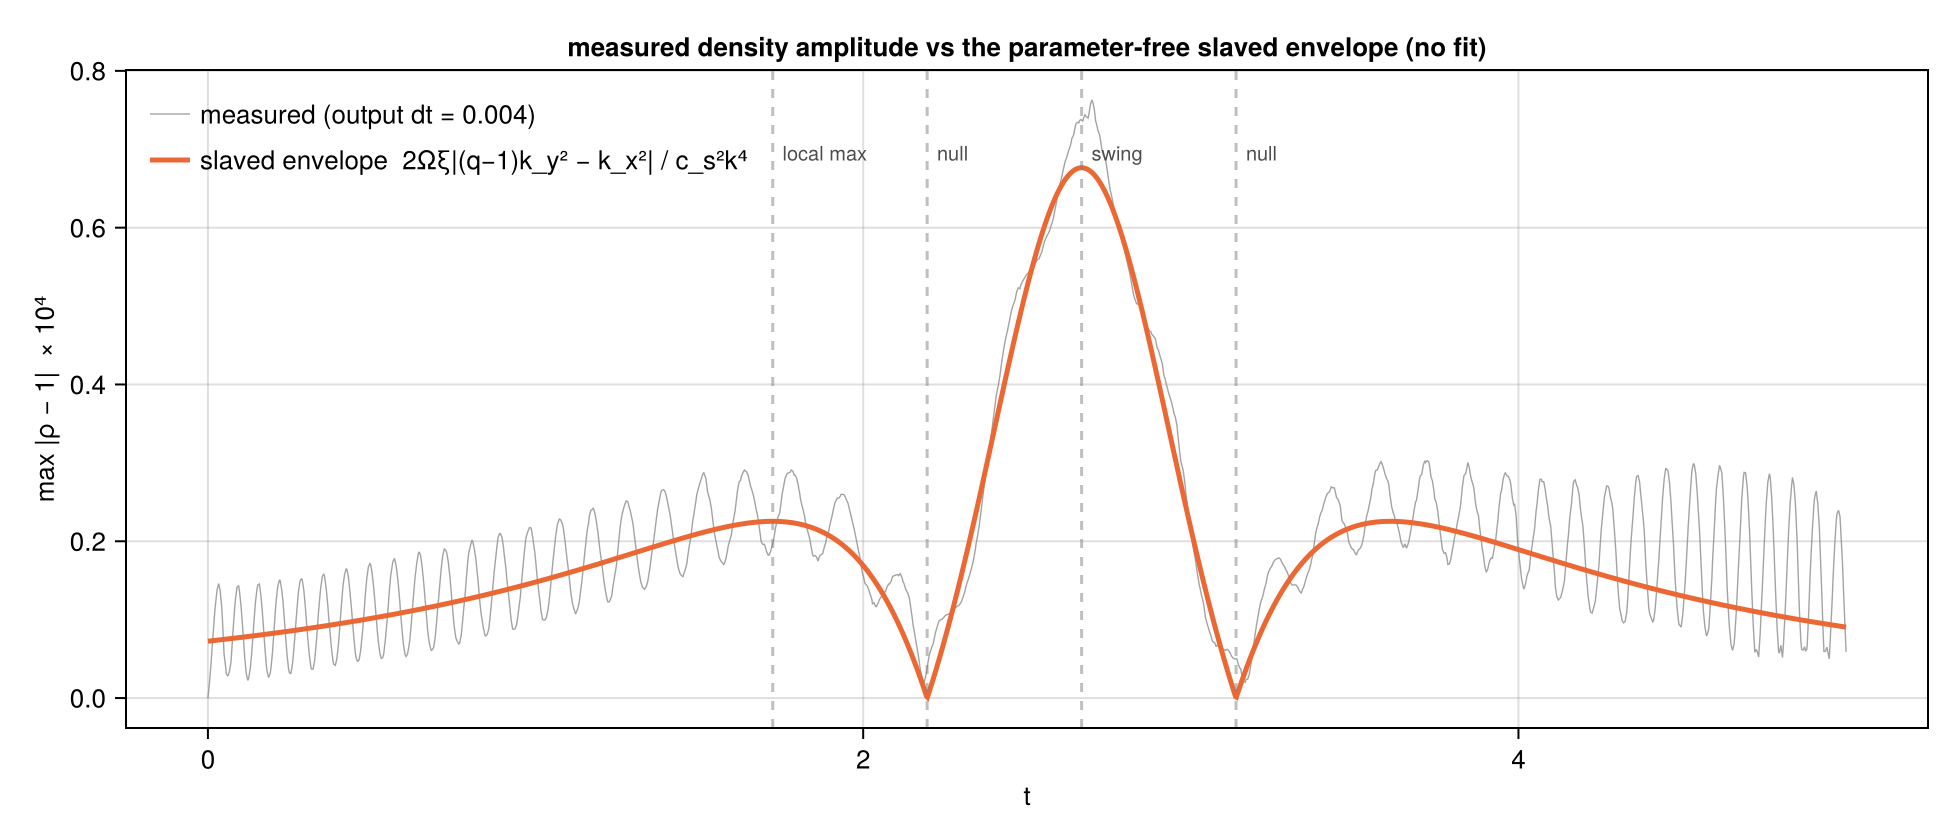
\includegraphics[width=\textwidth]{figures/pi_q02_envelope.png}
\caption{The measured density amplitude of the uniform vortical-shwave run
(gray; output $\dd t = 0.004$) against the slaved envelope of
Eq.~\eqref{eq:slaved} (orange) --- \emph{no fitted parameters}. Predicted local
max ($t=1.72$), nulls ($t=2.20$, $3.14$), swing peak ($t=2.67$,
$0.68\times10^{-4}$) and the $t^{-2}$ tail all line up; the fast oscillation
around the envelope is the free acoustic ringing.}
\end{figure}

\begin{figure}[htb]
\centering
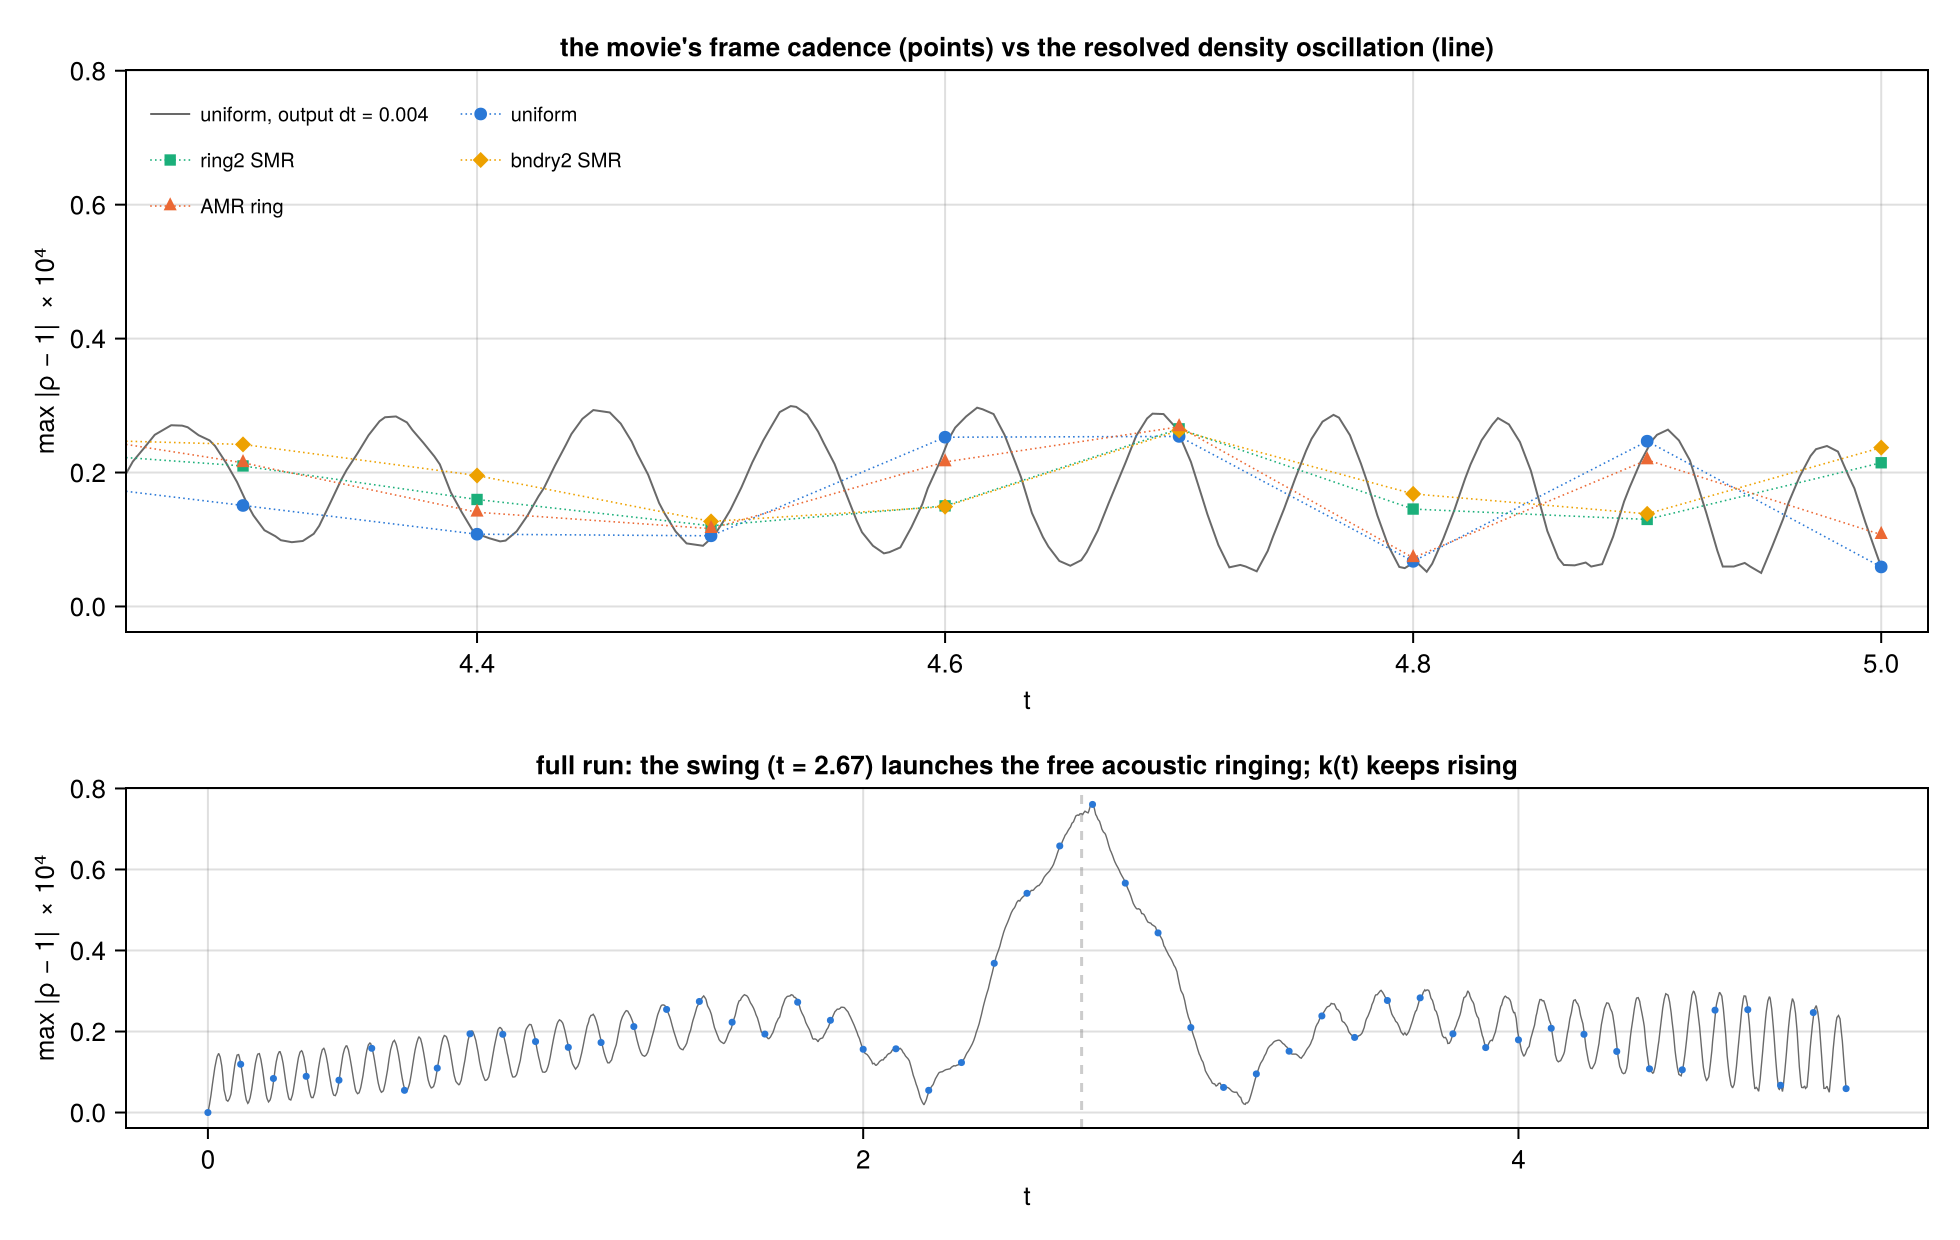
\includegraphics[width=\textwidth]{figures/pi_q02_alias.png}
\caption{Why the movie flickers: the four runs' 0.1-cadence frame samples
(points) hop across the resolved ringing (gray line) at quasi-random phases ---
2.4--2.9 beats of $|\rho - 1|$ elapse between consecutive frames near $t = 5$.
Bottom: full run; the ringing slows at the swing ($k$ minimum) and accelerates as
the wave rewinds.}
\end{figure}

%=====================================================================
\section*{References}
\begin{itemize}
\item[] Binney, J., \& Tremaine, S.\ 2008, \emph{Galactic Dynamics} (2nd ed.;
  Princeton), \S3.2.3 --- textbook epicycle theory behind \S\ref{sec:epi}.
\item[] Goldreich, P., \& Lynden-Bell, D.\ 1965, MNRAS, 130, 125 --- shearing
  waves and swing amplification.
\item[] Johnson, B.~M., \& Gammie, C.~F.\ 2005a, ApJ, 626, 978 --- linear
  ``shwave'' theory in the compressible shearing sheet; the linearized system of
  \S\ref{sec:shw} (\texttt{docs/Johnson\_2005\_ApJ\_626\_978.pdf}; cited by the
  \texttt{shwave.cpp} problem generator).
\item[] Johnson, B.~M., \& Gammie, C.~F.\ 2005b, ApJ, 635, 149 --- the vortical
  shwave as a code-verification test (their Fig.~1 and eq.~9)
  (\texttt{docs/Johnson\_2005\_ApJ\_635\_149.pdf}).
\item[] Bodo, G., et al.\ 2005, A\&A, 437, 9 --- density-wave emission by
  vortical perturbations in Keplerian shear (the slaved-response/ringing physics
  of \S\ref{sec:shw} in a broader setting).
\end{itemize}
\medskip
\noindent The derivations themselves are worked directly from the linearized
shearing-sheet equations (no formulas transcribed); the references anchor the
framework, the test problem, and the cross-checks.

\end{document}
